\chapter{Expanção em uma dimensão}
 Definido o método dos elementos finitos com a formulação de Galerkin, temos diferentes meios para resolver o problema. Anteriormente resolvemos uma equação diferencial usando elementos finitos com \textbf{equações lineares}. Discretizando o espaço em elementos de tamanho \textbf{h} e utilizando as técnicas de derivação e integração numérica utilizando polinômios de grau \textbf{p}, podemos utilizar a combinação desses métodos nos fornece aproximações com erros menores, para diferentes métodos.
 O método \textbf{p} utiliza um problema com um número de elementos fixo e para cada elemento usamos um  polinômio de grau \textbf{p} e verificamos a convergência do erro para cada grau desse polinômio. Temos o método \textbf{h} no qual fixamos o grau do polinômio e aumentamos o número de elementos, diminuindo o tamanho \textbf{h} de cada elemento.
 E o método espectral \textbf{hp} é a combinação de ambos os métodos anteriores, onde variamos o tamanho do elemento e o grau do polinômio para verificar a convergência do erro na obtenção de boas aproximações de uma função. 
 \section{Motivação do método hp}
 O método HP nos permite resolver problemas de geometrias complexas, no caso em uma dimensão casos com singularidades. Podemos verificar esse fenômenos em uma dimensão com a própria função de Runge anteriormente:
\begin{figure}[!h]
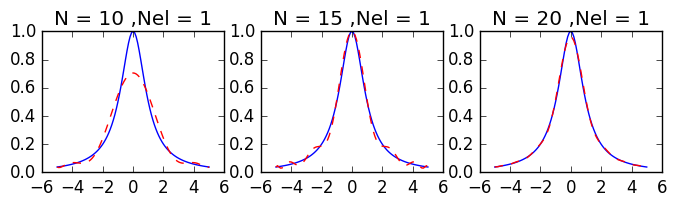
\includegraphics[width=0.6\textwidth, center ]{figuras/compara_metodo_n.png}
\caption{polinômio base de Lagrange para N  pontos em apenas um elemento}
\end{figure}
\\ Na figura acima vemos que para um problema subdividido em \emph{um} elemento, a aproximação acontece para um polinômio de lagrange de grau elevado, no caso anterior, n igual a 20. Porém  aumentando o número de elementos e tendo fixo o grau do polinômio, vemos que essa singularidade é contornada.

\begin{figure}[!b]
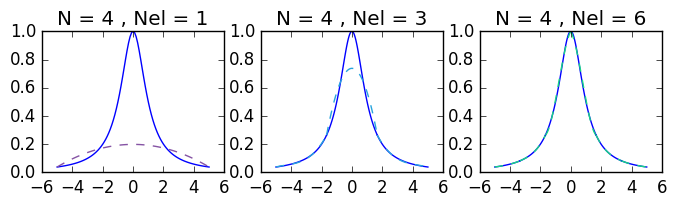
\includegraphics[width=0.6 \textwidth, center]{figuras/compara_metodo_n2.png}
\caption{Grau de polinômio fixo com diferentes números de elemento}
\end{figure}
\pagebreak
\subsection{[A decidir]}
	Ao decidir resolver a equação diferencial, obtemos um sistema de equações diferenciais para cada função teste $v_j^\delta$  e sem perder a igualdade transformamos o problema diferencial em um problema variacional, segue o exemplo abaixo:
\begin{align}
\frac{\partial^2 u^\delta }{\partial x^2} + \lambda u^\delta= f\\[1.5pt]
v^\delta_j (\frac{\partial^2 u^\delta }{\partial x^2} + \lambda v^\delta_j\ u^\delta) \ = v^\delta_j f\\[1.5pt]
\int_\Omega v^\delta_j (\frac{\partial^2 u^\delta }{\partial x^2} + \lambda v^\delta_j\  u^\delta) \partial x =\int_\Omega v^\delta_j  f \partial x\\[1.5pt]
\int_\Omega v^\delta_j \frac{\partial^2 u^\delta }{\partial x^2}\ \partial x + \int_\Omega \lambda v^\delta_j\ u^\delta\partial x =\ \int_\Omega v^\delta_j  f \partial x\\[1.5pt]
\int_\Omega \frac{\partial v^\delta_j }{\partial x} \frac{\partial u^\delta }{\partial x}\ \partial x + \int_\Omega \lambda v^\delta_j\ u^\delta\ \partial x - (v^\delta_j  \frac{\partial u^\delta }{\partial x})\Biggm\lvert_\Omega\ =\  \int_\Omega v^\delta_j\  f\ \partial x \ \forall j = 1,2,3,\dots,N 
\end{align}
 Como $u^\delta$ é a aproximada de $u$ utilizando a função teste $v^\delta_j$, temos:
\begin{align}
\sum^N_{i=1} u_i \int_\Omega \frac{\partial v^\delta_j }{\partial x} \frac{\partial v^\delta_i }{\partial x}\ \partial x +\sum^N_{i=1} u_i  \int_\Omega \lambda\ v^\delta_j v^\delta_i \ \partial x =\  (v^\delta_j  \frac{\partial u^\delta }{\partial x})\Biggm\lvert_\Omega + \int_\Omega v^\delta_j\ f\ \partial x \forall j =1,2,\dots,N 
\end{align}  
Como essa equação é definida para todo  $v_j$ para $j = 1,2,\dots,N$, podemos reescrever de forma matricial, onde $(v^\delta_j  \frac{\partial u^\delta }{\partial x})\Biggm\lvert_\Omega$ só é adicionado ao lado esquerdo quando se há uma condição de \emph{Neumann} e quando  $v^\delta_j$ é diferente de zero nos extremos do domínio. Assim, podemos reescrever o sistema como:
\begin{equation}
\{ M + \lambda S\} U = F
\end{equation}
\begin{align}
M &=
\begin{bmatrix}
\int_\Omega \frac{\partial v^\delta_{1}}{\partial x}\frac{\partial v^\delta_{1}}{\partial x}\ \partial x  & \int_\Omega \frac{\partial v^\delta_{1}}{\partial x}\frac{\partial v^\delta_{2}}{\partial x}\ \partial x  & \dots & \int_\Omega \frac{\partial v^\delta_{2}}{\partial x}\frac{\partial v^\delta_{N}}{\partial x}\ \partial x  \\ 
\int_\Omega \frac{\partial v^\delta_{1}}{\partial x}\frac{\partial v^\delta_{2}}{\partial x}\ \partial x  & \int_\Omega \frac{\partial v^\delta_{2}}{\partial x}\frac{\partial v^\delta_{2}}{\partial x}\ \partial x  & \dots & \int_\Omega \frac{\partial v^\delta_{2}}{\partial x}\frac{\partial v^\delta_{N}}{\partial x}\ \partial x  \\ 
\vdots & \vdots & \vdots & \dots \\
\int_\Omega \frac{\partial v^\delta_{N}}{\partial x}\frac{\partial v^\delta_{1}}{\partial x}\ \partial x  & \int_\Omega \frac{\partial v^\delta_{N}}{\partial x}\frac{\partial v^\delta_{2}}{\partial x}\ \partial x  & \dots & \int_\Omega \frac{\partial v^\delta_{N}}{\partial x}\frac{\partial v^\delta_{N}}{\partial x}\ \partial x  \\ 
\end{bmatrix} \\,
S &= \begin{bmatrix}
\int_\Omega v^\delta_1 v^\delta_1 \partial x & \int_\Omega v^\delta_1 v^\delta_2 \partial x & \dots & \int_\Omega v^\delta_1 v^\delta_N \partial x \\ 
\int_\Omega v^\delta_2 v^\delta_1 \partial x & \int_\Omega v^\delta_2 v^\delta_2 \partial x & \dots & \int_\Omega v^\delta_2 v^\delta_N \partial x\\ 
\vdots & \vdots & \ddots & \vdots \\
\int_\Omega v^\delta_N v^\delta_1 \partial x & \int_\Omega v^\delta_N v^\delta_2 \partial x & \dots & \int_\Omega v^\delta_N v^\delta_3 \partial x
\end{bmatrix},\
U = \begin{bmatrix}
u_1\\ 
u_2\\ 
\vdots \\
u_N
\end{bmatrix}\\
F &= \begin{bmatrix}
\int_\Omega v^\delta_1\ f\ \partial x +  (v^\delta_1  \frac{\partial u^\delta }{\partial x})\Biggm\lvert_\Omega \\ 
\int_\Omega v^\delta_2\ f\ \partial x +  (v^\delta_2  \frac{\partial u^\delta }{\partial x})\Biggm\lvert_\Omega \\ 
\vdots \\
\int_\Omega v^\delta_N\ f\ \partial x +  (v^\delta_N  \frac{\partial u^\delta }{\partial x})\Biggm\lvert_\Omega\\ 
\end{bmatrix}
\end{align}

\pagebreak

 
\subsection{Mapeamento}
 Quando tratamos das funções de bases, temos as funções globais e as locais. Apesar das funções globais serem na teoria usadas para o calcular as matrizes de \emph{massa} e de \emph{rigidez}, na prática decompomos as funções globais em elementos e utilizamos dessa decomposição as funções de base locais para o cálculo das matrizes.\\
 Tomemos como exemplo as funções lineares globais $\Phi$ em um domínio $\Omega = \{x\ |\ 0\leq x \leq 1\}$ subdividido em \emph{3} elementos. Temos 4 graus de liberdade nessa expansão, definida no máximo em 2 elementos ao mesmo tempo,que vale 1 em um dos extremos desses elementos e decresce para 0 para o em direção aos outros extremos.
\begin{equation}
\Phi_1(x) = \left\{\begin{matrix}
1 - 3x,\ 0 \leq x \leq \frac{1}{3}\\
0\ , \frac{1}{3} < x \leq 1
\end{matrix}\right.\ \ 
\Phi_2(x) = \left\{\begin{matrix}
3x,\ 0 \leq x \leq \frac{1}{3}\\
2 - 3x\ , \frac{1}{3} < x \leq \frac{2}{3}\\
0\ , \frac{2}{3} < x \leq 1
\end{matrix}\right.\\
\end{equation} 
\begin{equation}
\Phi_3(x) = \left\{\begin{matrix}
0 ,\ 0 \leq x < \frac{1}{3}\\
3x - 1\ ,\ \frac{1}{3} < x \leq \frac{2}{3}\\
-3x + 3 \ ,\ \frac{2}{3} < x \leq 1
\end{matrix}\right.\\
\Phi_4(x) = \left\{\begin{matrix}
0\ ,\ \ 0 \leq x < \frac{1}{3}\\
0\ ,\ \frac{1}{3} < x \leq \frac{2}{3}\\
3x -2 \ ,\ \frac{2}{3} < x \leq 1
\end{matrix}\right.
\end{equation}

\begin{figure}[!h]
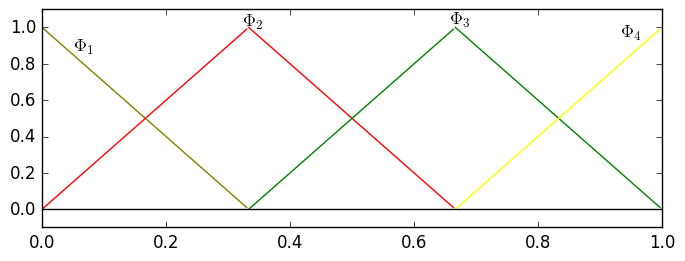
\includegraphics[width=0.6\textwidth, center ]{figuras/Matrix_elem_global.png}
\caption{funções globais para cada elemento}
\end{figure}

Também podemos definir funções locais $\phi^e_p(x)$ onde $\Omega_e = \{x \| x_{e1} \leq x \leq x_{e2} \}$:
\begin{equation}
\phi^e_1\ = \left\{\begin{matrix}
\frac{x_{e1}\ -\ x}{x_{e2} - x_{e1}}, x \in \Omega_e \\
0 ,\ x \notin \Omega_e 
\end{matrix}\right.
\phi^e_2\ = \left\{\begin{matrix}
\frac{x\ -\ x_{e1}}{x_{e2} - x_{e1}}, x \in \Omega_e \\
0 ,\ x \notin \Omega_e 
\end{matrix}\right.
\end{equation} 

\begin{figure}[!h]
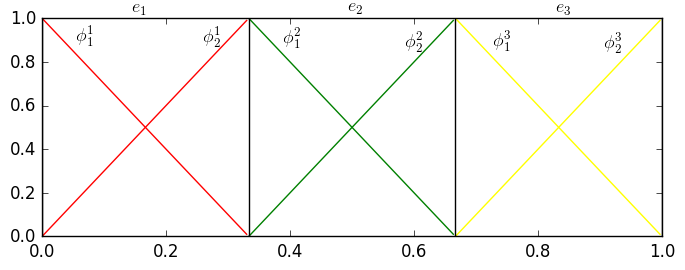
\includegraphics[width=0.6\textwidth, center ]{figuras/Matrix_element_local.png}
\caption{funções locais para cada elemento}
\end{figure}
 Podemos remapear $\Phi_i$'s em função das $\phi_i$'s locais como:
\begin{align}
\Phi_1 &= \phi_{1}^{1} \\[0.5pt]
\Phi_2 &= \phi_{2}^{1} + \phi_{1}^{2} \\[0.5pt]
\Phi_3 &= \phi_{2}^{2} + \phi_{1}^{3} \\[0.5pt]
\Phi_4 &= \phi_{2}^{3}
\end{align}

\begin{equation}
\begin{bmatrix}
\phi_1^1\\[1.9pt] 
\phi_2^1\\[1.9pt]
\phi_1^2\\[1.9pt] 
\phi_2^2\\[1.9pt]
\phi_1^3\\[1.9pt] 
\phi_2^3\\[1.9pt] 
\end{bmatrix}\ = \
\begin{bmatrix}
1 &0  & 0 & 0 \\ 
0 & 1 & 0 & 0\\ 
0 & 1 & 0 & 0\\ 
0 &0  & 1 & 0\\ 
0 &0  & 1 & 0\\ 
0 &0  & 0 & 1
\end{bmatrix}\
\begin{bmatrix}
\Phi_1\\ 
\Phi_2\\ 
\Phi_3\\ 
\Phi_4
\end{bmatrix}
\end{equation}

Notamos que existe uma relação entre as funções  $\Phi$ globais e as $\phi$ locais, para tal existe uma matriz $A$ que nos permite igualá-las, porém a relação inversa que nos mais interessa, na qual podemos fazer operações locais em cada elemento. Essa relação nos é interessante pois na formulação de Galerkin, nos permite fazer os cálculos das integrais localmente.
\begin{equation}
\int_\Omega\ \Phi_2(x) \partial x = \int_{0}^{\frac{1}{3}} \phi^1_2(x) \partial x + \int_{\frac{1}{3}}^{\frac{2}{3}} \phi^2_1(x)\ u(x) \partial x
\end{equation}

Devido ao fato da matriz $A$ ser uma matriz esparsa e portanto numericamente ineficiente para ser usada como um operador, utilizamos outra saída. Essa alternativa é uma matriz \emph{map}eadora em que cada coluna é um elemento (e) e cada linha o indice da função global (i).
\begin{equation}
map[1,i]= \begin{bmatrix}
1\\
2
\end{bmatrix},\
map[2,i]= \begin{bmatrix}
2\\
3
\end{bmatrix}\
,map[3,i]= \begin{bmatrix}
3\\
4
\end{bmatrix}
\end{equation}

usando um pseudo código, utilizamos essa matriz mapeadora para montar a função global dada a local:
\begin{lstlisting}
 for e =1:Nel
 	for i=1,2
 		$\Phi$[map[e,i]] = $\Phi$[map[e,i]] + $\phi$[e,i]
 	end
 end
\end{lstlisting}
Assim a matriz de massa \emph{global} $M$ definida como $M_{ij} = \int_\Omega \Phi_i\ \Phi_j \partial x$ analogamente como  o código anterior, pode ser reescrita a função de uma matriz de massa $M^e$ \emph{local}, utilizando uma matriz de mapeamento $map$ similar a anterior.
\begin{figure}[!h]
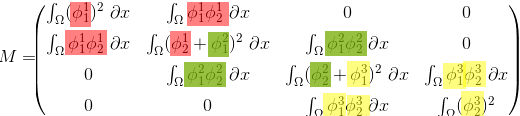
\includegraphics[width=0.6\textwidth, center ]{figuras/Matrix_element.png}
\caption{Matriz de massa mapeada}
\end{figure}